% =====================================================================
%  CLASE 01 -- Definiciones, propiedades de suelos, Ley de Darcy
% =====================================================================
\clase{01}{Hidrología subterránea: definiciones, propiedades de suelos y Ley de Darcy}

\section{Ocurrencia de agua subterránea}

Al estudiar el agua subterránea dentro del ciclo hidrológico surgen tres
preguntas fundamentales:
\begin{itemize}
  \item ¿Cómo llega el agua al suelo?
  \item ¿Cómo se transmite y almacena?
  \item ¿De qué factores dependerá?
\end{itemize}

\begin{figure}[H]
\centering
\begin{tikzpicture}[scale=0.9,font=\scriptsize]
  % terreno
  \fill[sueloclaro] (0,0) -- (0,2.2) -- (1.5,2.4) -- (3,4.2) -- (4.3,2.6)
        -- (6.5,2.0) -- (8.5,1.6) -- (10,1.2) -- (10,0) -- cycle;
  \fill[roca!70] (0,0) rectangle (10,0.6);
  \node[white] at (5,0.3) {Estratos impermeables};
  % oceano
  \fill[agua] (8.5,1.6) -- (10,1.2) -- (10,0.6) -- (8.3,0.6) -- cycle;
  \node at (9.3,1.0) {Océano};
  % nivel freático
  \draw[dashed,azulusm,thick] (0,1.6) .. controls (3,2.4) and (5,1.6) .. (8.5,1.3);
  \node[azulusm] at (4.6,1.95) {Nivel freático};
  % nubes y precipitación
  \foreach \x in {2,5.5,8.5}{
    \fill[gray!40] (\x,5.2) circle (0.35) (\x+0.4,5.3) circle (0.4) (\x+0.8,5.2) circle (0.35);
    \foreach \d in {0,0.3,0.6,0.9}
      \draw[agua,thick] (\x+\d-0.1,4.7) -- (\x+\d-0.25,4.35);}
  \node at (2.4,5.9) {Precipitación nival};
  \node at (5.9,5.9) {Precipitación pluvial};
  \node at (9.3,5.9) {Precipitación oceánica};
  % evaporación
  \draw[flecha,agua] (7.2,2.2) -- (7.2,3.4) node[right,black,align=left]{Evaporación y\\evapotranspiración};
  \draw[flecha,agua] (9.4,1.5) -- (9.4,3.9);
  % escorrentía y flujo subterráneo
  \draw[flecha,azulusm] (3.3,3.7) .. controls (4,2.8) .. (6,2.1) node[midway,above,sloped,black]{Escorrentía superficial};
  \draw[flecha,azulusm,dashed] (2,1.2) -- (7.5,1.0) node[midway,below,black]{Flujo subterráneo};
  \draw[flecha,azulusm] (1,2.3) -- (1,1.7) node[below,black]{Percolación};
  \node at (5,6.4) {\textbf{CICLO HIDROLÓGICO}};
\end{tikzpicture}
\caption{Esquema del ciclo hidrológico y ocurrencia del agua subterránea.}
\end{figure}

\section{Definiciones}

\subsection{Aguas subterráneas}
Agua existente bajo la superficie terrestre, que satura los intersticios
(``vacíos'') del terreno (``suelo'').

\begin{itemize}
  \item \textbf{Origen atmosférico}
  \item Proveniente de la \textbf{infiltración directa} de lluvias y nieves.
  \item \textbf{Aportes indirectos} de ríos y lagos.
  \item \textbf{Espesor de la zona capilar}:
  \begin{itemize}
    \item En suelos gruesos, arenas y gravas, del orden de mm o a lo más cm.
    \item En suelos finos, limos y principalmente arcillas, puede superar la
          decena de metros.
  \end{itemize}
\end{itemize}

\begin{figure}[H]
\centering
\begin{tikzpicture}[font=\small]
  % columna izquierda
  \fill[white] (0,0) rectangle (2.4,4);
  \fill[agua!25] (0,0) rectangle (2.4,1.6);
  \fill[agua] (2.4,0) rectangle (4.4,1.6);
  \fill[agua!25] (4.4,0) rectangle (6.8,1.6);
  \fill[gray!40] (0,-0.2) rectangle (6.8,0);
  \draw[dashed] (2.4,0) -- (2.4,4) (4.4,0) -- (4.4,4);
  \draw (0,4) -- (2.4,4) (4.4,4) -- (6.8,4);
  \draw[dashed] (0,2.6) -- (6.8,2.6);
  \draw[thick,azulusm] (0,1.6) -- (6.8,1.6);
  \foreach \i in {1,...,70}{
    \pgfmathsetmacro{\x}{rnd*2.3+0.05}\pgfmathsetmacro{\y}{rnd*1.5+0.05}
    \fill[azulusm] (\x,\y) circle (0.6pt);
    \fill[azulusm] (\x+4.4,\y) circle (0.6pt);}
  \foreach \i in {1,...,30}{
    \pgfmathsetmacro{\x}{rnd*2.3+0.05}\pgfmathsetmacro{\y}{rnd*2.3+1.65}
    \fill[black!60] (\x,\y) circle (0.5pt);
    \fill[black!60] (\x+4.4,\y) circle (0.5pt);}
  \node[align=center,font=\scriptsize] at (1.2,3.35) {Zona no aireación\\(agua y aire en poros)};
  \node[font=\scriptsize] at (1.2,2.1) {Zona capilar};
  \node[align=center,font=\scriptsize] at (1.2,0.8) {Zona saturada\\(sólo agua)};
  \node[font=\scriptsize] at (5.6,4.2) {Superficie};
  \node[font=\scriptsize] at (5.6,3.3) {Agua en el suelo};
  \node[font=\scriptsize] at (5.5,1.85) {Nivel freático};
  \pic at (6.55,1.62) {nivelagua};
  \node[font=\scriptsize] at (5.6,0.8) {Agua subterránea};
  \draw[decorate,decoration={brace,amplitude=5pt}] (-0.1,1.65) -- (-0.1,4)
     node[midway,left=6pt,align=center,font=\scriptsize]{Zona\\no saturada};
\end{tikzpicture}
\caption{Distribución vertical del agua en el subsuelo.}
\end{figure}

\subsection{Porosidad y porosidad efectiva}

\begin{itemize}
  \item \textbf{Porosidad:} máxima fracción volumétrica de agua en el suelo.
  \item \textbf{Porosidad efectiva:} fracción volumétrica que participa en el flujo.
\end{itemize}

\begin{formula}
$\displaystyle n=\frac{V_{\text{vacíos}}}{V_{\text{total}}}
\qquad\qquad
n_e=\frac{V_{\text{drenado}}}{V_{\text{total}}}$
\end{formula}

Valores típicos de porosidad según la estructura del suelo:
\begin{center}
\begin{tabular}{lc@{\hspace{1.5cm}}lc}
\toprule
Arena bien graduada & $n\approx 0.4$ & Arena mal graduada & $n\approx 0.2$\\
Arcilla sin compactar & $n\approx 0.7$ & Arcilla compactada & $n\approx 0.5$\\
\bottomrule
\end{tabular}
\end{center}

\begin{figure}[H]
\centering
\begin{minipage}{0.55\textwidth}
\centering
\begin{tikzpicture}
\begin{axis}[width=\linewidth,height=5.5cm,xmin=0,xmax=10,ymin=0,ymax=60,
  xticklabels={},xtick=\empty,ylabel={Volumen (\%)},xlabel={Tamaño del grano $\longrightarrow$},
  axis lines=left,font=\small,clip=false]
  \addplot[thick,black,smooth] coordinates {(0,52)(3,49)(6,45)(9,37)};
  \addplot[thick,black,smooth] coordinates {(0,47)(2,40)(4,25)(6,14)(9,6)};
  \addplot[thick,agua!80!black,smooth] coordinates {(0,4)(2,12)(4,24)(6,31)(7.5,33)(9,31)};
  \node[rojo,anchor=west,font=\scriptsize] at (axis cs:9.1,37){Porosidad};
  \node[rojo,anchor=west,font=\scriptsize,align=left] at (axis cs:9.1,30){Agua disponible\\para el flujo};
  \node[rojo,anchor=west,font=\scriptsize,align=left] at (axis cs:9.1,6){Agua no disponible\\para flujo};
\end{axis}
\end{tikzpicture}
\end{minipage}\hfill
\begin{minipage}{0.35\textwidth}
\centering
\begin{tabular}{lcc}
\toprule
Tipo de suelo & $n\,[\%]$ & $n_e\,[\%]$\\
\midrule
Arcillas & 50 & 4\\
Limos & 48 & 8\\
Arenas & 40 & 33\\
Gravas & 25 & 22\\
Rocas & $1\sim 8$ & $0.5\sim 4$\\
\bottomrule
\end{tabular}
\end{minipage}
\caption{Porosidad total, agua retenida (no disponible) y agua disponible
para el flujo en función del tamaño del grano.}
\end{figure}

\subsection{Clasificación de formaciones geológicas}
\begin{itemize}
  \item \textbf{Acuíferos}
  \begin{itemize}
    \item Formación geológica (gravas, arenas) que puede almacenar y transmitir
          agua (drenaje alto).
  \end{itemize}
  \item \textbf{Acuitardos}
  \begin{itemize}
    \item Formación geológica (limos, limos arcillosos, arcillas limosas) que
          puede almacenar, pero con mayor dificultad para transmitir agua
          (drenaje medio/bajo).
    \item Bajo condiciones especiales permiten una recarga vertical de otros acuíferos.
  \end{itemize}
  \item \textbf{Acuicludos}
  \begin{itemize}
    \item Formación geológica (arcillas, arcillas plásticas, limos arcillosos)
          con gran capacidad de almacenar, pero que no tiene posibilidad de
          transmitir (drenaje dificultoso).
  \end{itemize}
  \item \textbf{Acuífugos}
  \begin{itemize}
    \item Formación geológica impermeable (rocas), que no puede almacenar ni
          transmitir agua, salvo que existan fracturas que permitan flujos.
  \end{itemize}
\end{itemize}

\begin{table}[H]
\centering
\rowcolors{2}{azulusm!8}{white}
\begin{tabularx}{\textwidth}{l c c c X}
\toprule
\textbf{Tipo} & \textbf{Cap. almacenar} & \textbf{Cap. drenar} &
\textbf{Cap. transmitir} & \textbf{Formaciones características}\\
\midrule
Acuíferos  & Alta & Alta       & Alta & Gravas, arenas\\
Acuitardos & Alta & Media/Baja & Baja & Limos, limos arcillosos, arcillas limosas\\
Acuicludos & Alta & Muy baja   & Nula & Arcillas\\
Acuífugos  & Nula & Nula       & Nula & Rocas\\
\bottomrule
\end{tabularx}
\caption{Resumen de formaciones geológicas.}
\end{table}

Los que nos interesan son los \textbf{acuíferos}, caracterizados por su
\emph{extensión} (km$^2$) y su \emph{potencia} (m).

\begin{formula}
\textbf{Permeabilidad:} medida de la capacidad de un material poroso para transmitir agua.
\end{formula}

\section{Carga hidráulica y potencial piezométrico}

Antes de definir los tipos de acuíferos es necesario recordar la definición
de carga hidráulica. El nivel de energía en un punto se define utilizando la
ley de Bernoulli:
\begin{formula}
$\displaystyle H = z + \frac{p}{\gamma} + \frac{v^2}{2g}$
\end{formula}
Debido a que las velocidades en flujo subterráneo son bajas,
$\frac{v^2}{2g}\approx 0$, y por lo tanto:
\[
H = z + \frac{p}{\gamma} + \cancelto{\approx 0}{\frac{v^2}{2g}}
\quad\Longrightarrow\quad
\boxed{h = z + \frac{p}{\gamma}}\qquad h:\ \text{carga hidráulica}
\]

\begin{figure}[H]
\centering
\begin{tikzpicture}[font=\small]
  \draw[thick] (-1.5,4) -- (1.5,4);
  \fill[gray!20] (-1.5,0) rectangle (1.5,-0.2);
  \draw (-1.5,0) -- (1.5,0) node[right]{$z=0$};
  \draw (-0.15,1.2) rectangle (0.15,4.6);
  \fill[agua] (-0.15,1.2) rectangle (0.15,3.2);
  \draw[cota] (-0.8,0) -- (-0.8,3.2) node[midway,left]{$h$};
  \draw[cota] (0.7,0) -- (0.7,1.2) node[midway,right]{$z$};
  \draw[cota] (0.7,1.2) -- (0.7,3.2) node[midway,right]{$\dfrac{p}{\rho g}$};
  \draw[dashed] (-0.8,3.2) -- (0.7,3.2);
\end{tikzpicture}
\caption{Carga hidráulica medida en un piezómetro.}
\end{figure}

Para que exista flujo en un medio poroso se requiere la existencia de un
\textbf{gradiente de energía o potencial piezométrico}. El agua fluye desde
puntos de mayor carga $h_1$ hacia puntos de menor carga $h_2$.

\begin{figure}[H]
\centering
\begin{tikzpicture}[font=\small]
  \fill[pattern=crosshatch,pattern color=gray!50] (0,-0.3) rectangle (9,0);
  \draw (0,0) -- (9,0) node[right]{$z=0$};
  \draw (0,3.2) -- (4,3.2) (5,3.2) -- (9,3.2);
  \fill[agua] (4,0) rectangle (5,1.8);
  \draw (4,0) -- (4,3.2) (5,0) -- (5,3.2);
  \draw[dashed,azulusm,thick] (0,3.0) .. controls (2,2.9) and (3.5,2.3) .. (4,1.8);
  \draw[dashed,azulusm,thick] (5,1.8) .. controls (5.5,2.3) and (7,2.9) .. (9,3.0);
  \foreach \x/\h/\n in {0.8/2.95/1,2.4/2.65/2}{
    \draw (\x-0.12,1.0) rectangle (\x+0.12,3.5);
    \fill[agua] (\x-0.12,1.0) rectangle (\x+0.12,\h);
    \draw[cota] (\x-0.4,0) -- (\x-0.4,\h) node[midway,left]{$h_\n$};}
  \draw[flecha,azulusm] (1.4,0.8) -- (2.0,0.8);
\end{tikzpicture}
\caption{El flujo se produce en la dirección de disminución de la carga hidráulica ($h_1>h_2$).}
\end{figure}

\section{Tipos de acuíferos}

\begin{itemize}
  \item \textbf{Acuífero libre:} cercanos a la superficie terrestre; su límite
        superior es el nivel freático (superficie con presión atmosférica).
  \item \textbf{Acuífero artesiano o confinado:} confinados entre estratos
        impermeables, por ende, bajo presión.
  \item \textbf{Acuífero semi-confinado:}
  \begin{itemize}
    \item Confinados entre estratos semi-permeables.
    \item Bajo presión, pero una o ambas capas permiten alguna filtración.
  \end{itemize}
\end{itemize}

\begin{figure}[H]
\centering
\begin{tikzpicture}[font=\scriptsize,scale=1.0]
  % capa impermeable inferior
  \fill[suelo!80!black] (0,0) rectangle (11,0.8);
  \node at (7,0.4) {Capa impermeable};
  % acuífero cautivo
  \fill[gray!45] (0,0.8) -- (11,0.8) -- (11,1.9) .. controls (7,1.9) and (4,1.5) .. (1.5,4.0) -- (0,4.0) -- cycle;
  \node at (6.5,1.3) {Acuífero cautivo (confinado)};
  % capa confinante
  \fill[suelo] (1.5,4.0) .. controls (4,1.5) and (7,1.9) .. (11,1.9) -- (11,2.2)
      .. controls (7,2.2) and (4.2,1.9) .. (2.0,4.3) -- cycle;
  \node at (4.2,2.05) {Capa confinante};
  % acuífero libre
  \fill[agua!40] (2.0,4.3) .. controls (4.2,1.9) and (7,2.2) .. (11,2.2) -- (11,3.3) -- (3.3,3.3) -- cycle;
  \node at (9.2,2.7) {Acuífero libre};
  % zona no saturada
  \fill[sueloclaro] (3.3,3.3) -- (11,3.3) -- (11,4.0) .. controls (8,4.2) and (6,3.8) .. (4,4.4) -- (2.0,4.3) -- cycle;
  \draw[dashed] (0,3.5) -- (11,3.5);
  \node[align=center] at (0.9,3.7) {Nivel de agua\\subterránea};
  \node at (9.8,3.55) {Nivel freático};
  % zona de recarga
  \fill[sueloclaro] (0,4.0) -- (1.5,4.0) -- (2.0,4.3) -- (0,4.9) -- cycle;
  \foreach \x in {0.3,0.6,0.9,1.2}
    \draw[flecha,rojo] (\x,5.7) -- (\x,4.9);
  \node at (0.8,5.95) {Zona de recarga};
  % pozos
  \draw[line width=2pt,azulusm] (4.8,4.1) -- (4.8,1.2);
  \foreach \a in {60,90,120} \draw[azulusm] (4.8,4.1) -- ++(\a:0.4);
  \node[align=center] at (4.8,4.85) {Pozo artesiano\\surgente};
  \draw[line width=2pt,azulusm] (8.0,4.1) -- (8.0,1.2);
  \node[align=center] at (8.0,4.85) {Pozo artesiano\\no surgente};
\end{tikzpicture}
\caption{Acuífero libre y acuífero confinado (cautivo). El nivel piezométrico
del acuífero confinado puede quedar sobre el terreno (pozo surgente).}
\end{figure}

\begin{figure}[H]
\centering
\begin{tikzpicture}[font=\small]
  \fill[pattern=crosshatch,pattern color=black!60] (0,0) rectangle (8,0.3);
  \node[fill=white,inner sep=1pt] at (7,0.15) {Impermeable};
  \fill[sueloclaro] (0,0.3) rectangle (8,1.6);
  \node at (1.8,0.95) {Acuífero semiconfinado};
  \fill[gray!35] (0,1.6) rectangle (8,2.4);
  \node at (1.8,2.0) {Acuitardo};
  \fill[agua!25] (0,2.4) rectangle (8,3.4);
  \node at (1.8,2.9) {Acuífero libre};
  \fill[sueloclaro!60] (0,3.4) rectangle (8,4.2);
  \draw[thick,azulusm] (0,3.4) -- (8,3.4) node[right,align=left,font=\scriptsize,yshift=-6pt]{Superficie freática\\(acuífero libre superior)};
  \draw[thick,rojo,dashed] (0,3.7) -- (8,3.7) node[right,align=left,font=\scriptsize,yshift=10pt]{Superficie piezométrica\\(acuífero semiconfinado)};
  \foreach \x in {3.5,5,6.5} \draw[flecha,azulusm] (\x,2.35) -- (\x,1.65);
\end{tikzpicture}
\caption{Acuífero semiconfinado: la recarga vertical ocurre a través del acuitardo.}
\end{figure}

\section{Explotación de acuíferos}

Para poder aprovechar los recursos de aguas subterráneas es necesario que
ésta aflore a la superficie. Para esto se presentan dos alternativas:
\begin{itemize}
  \item \textbf{Vertientes:} lugares donde, debido a la configuración geológica
        y geomorfológica de los suelos, el agua aflora naturalmente a la superficie.
  \item \textbf{Pozos o drenes.}
\end{itemize}

\subsection{Tipos de vertientes}
\begin{itemize}
  \item \textbf{Vertientes de depresión:} generalmente cajones de ríos.
  \item \textbf{Vertientes de contacto.}
  \item \textbf{Vertientes de fractura:} normalmente en zonas cordilleranas.
  \item \textbf{Vertientes de dique.}
\end{itemize}

\begin{figure}[H]
\centering
\begin{subfigure}{0.48\textwidth}\centering
\begin{tikzpicture}[scale=0.75,font=\scriptsize]
  \fill[top color=agua!30,bottom color=azulusm!80] (0,0) -- (0,3) -- (2.8,3) -- (3.6,2.4) -- (4.4,2.4) -- (5.2,3) -- (8,3) -- (8,0) -- cycle;
  \fill[gray!25] (0,3) -- (0,3.4) -- (2.2,3.4) -- (3.4,2.55) -- (2.8,3) -- cycle;
  \fill[gray!25] (8,3) -- (8,3.4) -- (5.8,3.4) -- (4.6,2.55) -- (5.2,3) -- cycle;
  \draw (0,3.4) -- (2.2,3.4) -- (3.4,2.55) .. controls (3.8,2.3) and (4.2,2.3) .. (4.6,2.55) -- (5.8,3.4) -- (8,3.4);
  \foreach \x in {0.3,0.8,...,2.0} \draw[flecha] (\x,4.1) -- (\x,3.45);
  \foreach \x in {6.0,6.5,...,7.8} \draw[flecha] (\x,4.1) -- (\x,3.45);
  \draw[impermeable] (0,-0.3) rectangle (8,0);
  \draw[<-] (4.4,2.45) -- (6,2.2) node[right]{Recuperación};
\end{tikzpicture}
\caption{Vertiente de depresión.}
\end{subfigure}\hfill
\begin{subfigure}{0.48\textwidth}\centering
\begin{tikzpicture}[scale=0.75,font=\scriptsize]
  \fill[gray!30] (0,0) -- (1.5,0) -- (2.5,1.3) -- (7,1.3) -- (7,0) -- cycle;
  \fill[gray!10,draw=black] (2.5,1.3) -- (7,1.3) -- (7,1.8) -- (2.2,1.6) -- cycle;
  \fill[agua] (2.2,1.6) -- (7,1.8) -- (7,2.4) -- (4,2.2) -- cycle;
  \fill[gray!30] (2.2,1.6) -- (4,2.2) -- (7,2.4) -- (7,3.6) -- (5,3.4) -- cycle;
  \draw (1.5,0) -- (2.5,1.3) (2.2,1.6) -- (5,3.4) -- (7,3.6) -- (7,0);
  \fill[agua] (2.2,1.6) -- (1.7,1.75) -- (2.0,1.5) -- cycle;
  \draw[<-] (2.0,1.7) -- (1.3,2.6) node[above]{Afloramiento de agua};
  \draw[<-] (7,1.55) -- (7.6,1.2) node[below]{Material impermeable};
  \draw[<-] (5.8,3.5) -- (6.2,4.1) node[above]{Superficie del suelo};
\end{tikzpicture}
\caption{Vertiente de contacto.}
\end{subfigure}

\medskip
\begin{subfigure}{0.48\textwidth}\centering
\begin{tikzpicture}[scale=0.75,font=\scriptsize]
  \fill[azulusm!70] (1.2,0) -- (1.2,0.4) -- (8,2.5) -- (8,0) -- cycle;
  \fill[gray!25] (1.2,0.4) -- (8,2.5) -- (8,4) -- (5,3.3) -- (3,2.6) -- (1.3,0.6) -- cycle;
  \draw[thick,gray] (1.3,0.6) -- (3,2.6) -- (5,3.3) -- (8,4);
  \foreach \a/\b in {3.0/2.5,4.5/3.1,6/3.6,7.2/3.9}
     \draw[azulusm] (\a,\b) -- (\a+0.7,\b-1.6);
  \fill[agua] (1.2,0.5) -- (0.6,0.8) -- (0.8,0.4) -- cycle;
  \node[above] at (0.8,1.2) {Afloramiento};
  \node at (4.5,4.0) {Fracturas};
  \node[right] at (5.8,4.5) {Material impermeable};
\end{tikzpicture}
\caption{Vertiente de fractura.}
\end{subfigure}\hfill
\begin{subfigure}{0.48\textwidth}\centering
\begin{tikzpicture}[scale=0.75,font=\scriptsize]
  \fill[gray!40] (0,0) rectangle (8,1.2);
  \fill[agua] (0.3,1.8) .. controls (1.5,0.4) and (2.6,0.4) .. (3.3,1.8) -- cycle;
  \fill[agua] (5.2,1.8) .. controls (5.8,0.3) and (7,0.3) .. (7.7,1.8) -- cycle;
  \fill[sueloclaro] (0.3,1.8) -- (3.3,1.8) -- (3.5,2.1) -- (0.2,2.0) -- cycle;
  \fill[sueloclaro] (5.2,1.8) -- (7.7,1.8) -- (7.8,2.2) -- (5,2.1) -- cycle;
  \fill[gray!40] (0,1.2) -- (0,1.9) .. controls (1.5,0.2) and (2.8,0.2) .. (3.4,1.8)
      -- (4.2,4) -- (5.1,1.8) .. controls (5.8,0) and (7,0) .. (8,2.2) -- (8,1.2) -- cycle;
  \node at (4.2,1.8) {Roca basal};
  \fill[agua] (0,1.9) -- (-0.5,2.1) -- (-0.3,1.8) -- cycle;
  \node[above] at (-0.2,2.2) {Afloramiento};
  \node at (1.3,0.6) {``Ojo de agua''};
  \node[above] at (6.5,2.3) {Material permeable};
\end{tikzpicture}
\caption{Vertiente de dique.}
\end{subfigure}
\caption{Tipos de vertientes.}
\end{figure}

\section{Ley de Darcy (1856)}

Darcy observó experimentalmente, en un tubo lleno de arena, que el caudal
$Q$ que atraviesa la muestra cumple:
\[
Q\propto A,\qquad Q\propto \Delta h,\qquad Q\propto\frac{1}{L}
\]
de donde:
\begin{formula}
$\displaystyle Q=-K\cdot A\cdot\left(\frac{\dd h}{\dd l}\right)=-K\cdot A\cdot i$\\[4pt]
\textbf{Ley de Darcy} --- válida para flujo laminar ($Re<4$)
\end{formula}

\begin{figure}[H]
\centering
\begin{minipage}{0.5\textwidth}\centering
\begin{tikzpicture}[scale=0.85,font=\small]
  \draw (-0.5,0) -- (5.5,0) node[right]{$z=0$};
  % tubo inclinado
  \begin{scope}
    \fill[agua!60] (0.9,4.2) -- (1.3,4.6) -- (4.1,1.8) -- (3.7,1.4) -- cycle;
    \draw (0.9,4.2) -- (3.7,1.4) (1.3,4.6) -- (4.1,1.8);
    \foreach \i in {1,...,60}{\pgfmathsetmacro{\t}{rnd}\pgfmathsetmacro{\s}{rnd}
      \fill[azulusm] ({0.9+2.8*\t+0.4*\s*0.7},{4.2-2.8*\t+0.4*\s*0.7}) circle (0.6pt);}
  \end{scope}
  % piezómetros
  \fill[agua] (1.05,4.35) rectangle (1.35,5.6);
  \draw (1.05,4.35) -- (1.05,6.0) (1.35,4.5) -- (1.35,6.0);
  \fill[agua] (3.85,1.65) rectangle (4.15,5.2);
  \draw (3.85,1.8) -- (3.85,6.0) (4.15,1.9) -- (4.15,6.0);
  \draw[dashed] (0,5.6) -- (5,5.6) (3.6,5.2) -- (5,5.2);
  \draw[cota] (0.2,0) -- (0.2,5.6) node[midway,left]{$h_1$};
  \draw[cota] (0.6,0) -- (0.6,4.4) node[midway,left]{$z_1$};
  \draw[cota] (4.9,0) -- (4.9,5.2) node[midway,right]{$h_2$};
  \draw[cota] (4.5,0) -- (4.5,1.8) node[midway,right]{$z_2$};
  \draw[cota] (5.3,5.2) -- (5.3,5.6) node[midway,right]{$\Delta h$};
  \draw[cota] (0.6,3.6) -- (3.3,0.9) node[midway,below left]{$L$};
  \draw[flecha,azulusm] (1.4,3.9) -- (2.2,3.1);
\end{tikzpicture}
\end{minipage}\hfill
\begin{minipage}{0.45\textwidth}\centering
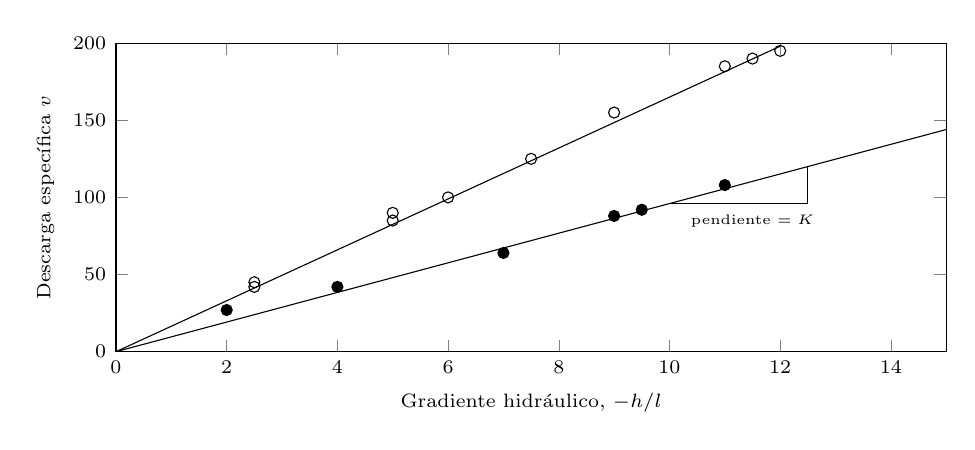
\begin{tikzpicture}
\begin{axis}[width=\linewidth,height=5.5cm,xmin=0,xmax=15,ymin=0,ymax=200,
  xlabel={Gradiente hidráulico, $-\dd h/\dd l$},ylabel={Descarga específica $v$},font=\scriptsize]
  \addplot[only marks,mark=o] coordinates {(2.5,45)(2.5,42)(5,85)(5,90)(6,100)(7.5,125)(9,155)(11,185)(11.5,190)(12,195)};
  \addplot[only marks,mark=*] coordinates {(2,27)(4,42)(7,64)(9,88)(9.5,92)(11,108)};
  \addplot[domain=0:12,samples=2] {16.5*x};
  \addplot[domain=0:15,samples=2] {9.6*x};
  \draw (axis cs:10,96) -- (axis cs:12.5,96) -- (axis cs:12.5,120);
  \node[font=\tiny] at (axis cs:11.5,85) {pendiente $=K$};
\end{axis}
\end{tikzpicture}
\end{minipage}
\caption{Experimento de Darcy: la descarga específica es proporcional al
gradiente hidráulico, siendo la pendiente la conductividad hidráulica $K$.}
\end{figure}

\subsection{Generalización de la Ley de Darcy}

Generalmente, en un suelo estratificado la resistencia al flujo no es igual
en todas direcciones $\Rightarrow$ \textbf{medio anisotrópico}:
\begin{formula}
$\vec v=-\mathbf{K}\,\nabla h$
\end{formula}
con
\[
\vec v=v_x\hat\imath+v_y\hat\jmath+v_z\hat k,\qquad
\nabla h=\frac{\partial h}{\partial x}\hat\imath+\frac{\partial h}{\partial y}\hat\jmath+\frac{\partial h}{\partial z}\hat k,\qquad
\mathbf K=\begin{pmatrix}K_{xx}&K_{xy}&K_{xz}\\K_{yx}&K_{yy}&K_{yz}\\K_{zx}&K_{zy}&K_{zz}\end{pmatrix}
\]
\begin{itemize}
  \item Si la dirección principal de anisotropía coincide con $x,y,z$:
  \[K_{xy}=K_{yx}=K_{xz}=K_{zx}=K_{yz}=K_{zy}=0\]
  \item Si no hay dirección de flujo preferente (\textbf{medio isotrópico}):
  \[K_x=K_y=K_z=K\]
\end{itemize}

\section{Conductividad hidráulica, $K$}
\begin{itemize}
  \item También conocida como \textbf{coeficiente de permeabilidad}.
  \item Unidades L/T, comúnmente expresada en cm/s.
  \item Función de las propiedades del medio poroso y del fluido.
\end{itemize}
\begin{formula}
$\displaystyle K=k\,\frac{\rho g}{\mu}=k\,\frac{\gamma}{\mu}$
\qquad $k$: permeabilidad intrínseca [darcy],\quad
1 darcy $=9.87\times10^{-9}$ cm$^2$
\end{formula}

\begin{table}[H]
\centering
\begin{tabular}{lcc}
\toprule
\textbf{Material} & \textbf{Permeabilidad intrínseca $k$ [darcy]} & \textbf{Conductividad $K$ [cm/s]}\\
\midrule
Arcilla & $10^{-6}$ -- $10^{-3}$ & $10^{-9}$ -- $10^{-6}$\\
Limo, limos arenosos, arenas arcillosas & $10^{-3}$ -- $10^{-1}$ & $10^{-6}$ -- $10^{-4}$\\
Arenas limosas, arenas finas & $10^{-2}$ -- $1$ & $10^{-5}$ -- $10^{-3}$\\
Arenas bien distribuidas & $1$ -- $10^{2}$ & $10^{-3}$ -- $10^{-1}$\\
Gravas bien distribuidas & $10$ -- $10^{3}$ & $10^{-2}$ -- $1$\\
\bottomrule
\end{tabular}
\caption{Valores típicos de permeabilidad intrínseca y conductividad hidráulica.}
\end{table}

\subsection{Factores de los suelos que condicionan $K$}
\begin{itemize}
  \item \textbf{Porosidad efectiva.}
  \item \textbf{Forma de los granos:} esférica, tubular o prismática, laminar
        ($K$ aumenta desde laminar hacia esférica).
  \item \textbf{Granulometría:} I.~material homogéneo; II.~material heterogéneo.
        Se cumple $K_I>K_{II}$.
  \item \textbf{Presencia de material fino} (pasante bajo malla 200,
        0.074~mm): si se presenta un 12\% a 15\% de material bajo esta malla,
        el material presenta una mala permeabilidad.
  \item Viscosidad del agua.
  \item Grado de saturación del suelo.
  \item En el caso de las arcillas también influyen:
  \begin{itemize}
    \item La estructura.
    \item La concentración iónica.
    \item Espesor de capas de agua adheridas a las partículas de arcilla.
  \end{itemize}
  \item Para un material arenoso o gravoso, que sea mal graduado indica que
        posee una mayor cantidad de limos o arcillas.
  \item Las arcillas no se consideran bien o mal graduadas.
\end{itemize}

\begin{figure}[H]
\centering
\begin{tikzpicture}[font=\small]
  \draw[flecha] (0,0) -- (6,0) node[right]{$D$};
  \draw[flecha] (0,0) -- (0,3.5) node[left]{\%};
  \draw[azulusm] (0,3) -- (5.5,3);
  \draw[thick] (0,0) .. controls (1.5,0.3) and (2,2.9) .. (3,3) -- (5,3);
  \draw[thick,dashed] (0,0) .. controls (2.5,0.2) and (3.5,2) .. (4.6,3) -- (5,3);
  \node at (1.8,1.8) {I};
  \node at (3.3,1.5) {II};
  \node[rojo] at (0.9,2.4) {Homogéneo};
  \node[rojo] at (5,1.2) {Heterogéneo};
  \node at (2.5,-0.5) {$K_I>K_{II}$};
  \node[azulusm] at (3,3.35) {Curvas granulométricas};
\end{tikzpicture}
\caption{Curvas granulométricas: material homogéneo (I) y heterogéneo (II).}
\end{figure}

\section{Métodos indirectos para determinar $K$}

\subsection{Información bibliográfica o empírica}
Depende del tipo de suelo; existen tablas de rangos de permeabilidad
intrínseca y conductividad hidráulica por tipo de material (p.~ej.\ Freeze
\& Cherry, 1979): desde rocas ígneas no fracturadas ($K\sim10^{-11}$ cm/s)
hasta gravas y calizas kársticas ($K\sim 10^{0}$--$10^{2}$ cm/s).

\subsection{Método de Hazen}
En suelos arenosos, a partir de la curva granulométrica, para arenas con
$d_{10}$ entre 0.1 y 0.3~mm:
\begin{formula}
$K=C\cdot(d_{10})^2\ \ [\text{cm/s}],\qquad d_{10}$ en [cm]
\end{formula}
\begin{table}[H]
\centering
\begin{tabular}{lc}
\toprule
\textbf{Tipo de arena} & $C$\\
\midrule
Arena muy fina, mal distribuida & 40 -- 80\\
Arena fina con una gran cantidad de material fino & 40 -- 80\\
Arena media, bien distribuida & 80 -- 120\\
Arena gruesa, mal distribuida & 80 -- 120\\
Arena gruesa, bien distribuida, limpia & 120 -- 150\\
\bottomrule
\end{tabular}
\end{table}

\subsection{Método de Slichter}
Basado en curva granulométrica y porosidad:
\[
K=\frac{\gamma}{\mu}\,\frac{10.0219\cdot d_{10}^2}{K_1},\qquad d_{10}\ \text{en [cm]}
\]
\begin{table}[H]
\centering
\begin{tabular}{cc@{\hspace{1cm}}cc}
\toprule
$n$ & $1/K_1$ & $n$ & $1/K_1$\\
\midrule
0.26 & 0.00187 & 0.38 & 0.04154\\
0.28 & 0.01517 & 0.40 & 0.04922\\
0.30 & 0.01905 & 0.42 & 0.05789\\
0.32 & 0.02356 & 0.44 & 0.06776\\
0.34 & 0.02878 & 0.46 & 0.07838\\
0.36 & 0.03473 & & \\
\bottomrule
\end{tabular}
\end{table}

\subsection{Método de Kozeny--Carman}
\[
K=\left(\frac{\rho g}{\mu}\right)\cdot\left[\frac{n^3}{(1-n^2)}\right]\cdot\left(\frac{d_{50}^2}{180}\right)
\]
con $\mu$: viscosidad; $n$: porosidad; $d_{50}$ en [cm].

\section{Métodos directos para determinar $K$}

\subsection{Pruebas de laboratorio}
La conductividad hidráulica de un suelo saturado se mide mediante
\textbf{permeámetros}.

\paragraph{Permeámetro de carga constante}
\begin{itemize}
  \item Sedimentos no cohesivos, arenas, rocas.
  \item Se alcanza una situación de equilibrio.
  \item Utilizar gradientes hidráulicos similares a los existentes en terreno.
  \item $h_1-h_2<50\%\,L$.
\end{itemize}
\begin{formula}
$\displaystyle K=\frac{4\cdot L\cdot Q}{\pi\cdot(h_1-h_2)\cdot D^2}$
\end{formula}

\paragraph{Permeámetro de carga variable}
\begin{itemize}
  \item Sedimentos cohesivos con baja permeabilidad.
\end{itemize}
\begin{formula}
$\displaystyle K=\frac{d_t^2\cdot L}{d_c^2\cdot t}\cdot\ln\!\left(\frac{h_0}{h}\right)$
\qquad $d_t$: diámetro del tubo;\ $d_c$: diámetro de la muestra
\end{formula}

\begin{figure}[H]
\centering
\begin{subfigure}{0.48\textwidth}\centering
\begin{tikzpicture}[scale=0.8,font=\small]
  % estanque superior
  \draw (2,5) rectangle (3,6.2); \fill[agua] (2,5) rectangle (3,5.9);
  \draw[thick] (2.3,6.2) -- (2.3,6.6) -- (3.3,6.6) node[right,rojo]{Entrada};
  \draw[thick] (3,5.9) -- (3.6,5.9) -- (3.6,5.6) node[below,rojo]{Descarga};
  % tubo de conexión
  \draw[line width=3pt,agua] (2.9,5) -- (2.9,0.2) -- (2.2,0.2);
  % muestra
  \draw (1,0) rectangle (2.2,2.5); \fill[agua] (1,0) rectangle (2.2,2.2);
  \fill[pattern=north east lines] (1,0.4) rectangle (2.2,0.55);
  \fill[pattern=north east lines] (1,1.75) rectangle (2.2,1.9);
  \foreach \i in {1,...,30}\fill[azulusm!70!black] ({1.05+1.1*rnd},{0.6+1.1*rnd}) circle (0.7pt);
  \node[font=\scriptsize,align=center] at (1.6,1.15) {Muestra};
  \draw[thick] (1,2.2) -- (0.4,2.2) -- (0.4,1.9);
  \fill[agua] (-0.2,0) rectangle (0.8,0.8); \draw (-0.2,0) rectangle (0.8,1.1);
  \draw[dashed] (-0.6,5.9) -- (2,5.9) node[pos=0,left]{$h_1$};
  \draw[dashed] (-0.6,2.2) -- (0.4,2.2) node[pos=0,left]{$h_2$};
  \draw[cota] (2.5,2.2) -- (2.5,5.9) node[midway,left]{$h_1-h_2$};
  \draw[cota] (0.8,0.55) -- (0.8,1.75) node[midway,left]{$L$};
  \draw[cota] (1,-0.3) -- (2.2,-0.3) node[midway,below]{$D$};
  \node[rojo,align=center] at (4.3,1.7) {Placas\\porosas};
\end{tikzpicture}
\caption{Carga constante.}
\end{subfigure}\hfill
\begin{subfigure}{0.48\textwidth}\centering
\begin{tikzpicture}[scale=0.8,font=\small]
  \draw (1,0) rectangle (2.5,3);
  \fill[agua] (1,0) rectangle (2.5,2.7);
  \fill[pattern=north east lines] (1,0.4) rectangle (2.5,0.55);
  \fill[pattern=north east lines] (1,1.9) rectangle (2.5,2.05);
  \foreach \i in {1,...,30}\fill[azulusm!70!black] ({1.05+1.4*rnd},{0.6+1.25*rnd}) circle (0.7pt);
  \node[font=\scriptsize,align=center] at (1.75,1.2) {Muestra};
  % tubo delgado
  \draw (3.2,0.2) -- (3.2,5.5) (3.4,0.2) -- (3.4,5.5);
  \fill[agua] (3.2,0.2) rectangle (3.4,3.5);
  \draw[line width=2pt,agua] (2.5,0.15) -- (3.3,0.15);
  \draw[thick] (1,2.7) -- (0.2,2.7) -- (0.2,2.4);
  \fill[agua] (-0.3,0) rectangle (0.7,0.9); \draw (-0.3,0) rectangle (0.7,1.2);
  \draw[dashed] (1.7,5) -- (3.2,5) (1.7,2.7) -- (1,2.7) (2.5,3.5) -- (3.2,3.5);
  \draw[cota] (1.7,2.7) -- (1.7,5) node[midway,left]{$h_0$};
  \draw[cota] (2.8,2.7) -- (2.8,3.5) node[midway,left]{$h$};
  \draw[cota] (0.8,0.55) -- (0.8,1.9) node[midway,left]{$L$};
  \draw[cota] (1,-0.3) -- (2.5,-0.3) node[midway,below]{$d_c$};
  \draw[->] (2.8,5.8) -- (3.2,5.8); \draw[<-] (3.4,5.8) -- (3.8,5.8) node[right]{$d_t$};
  \node[rojo,align=center] at (4.6,1.9) {Placas\\porosas};
\end{tikzpicture}
\caption{Carga variable.}
\end{subfigure}
\caption{Permeámetros de laboratorio.}
\end{figure}

\subsection{Mediciones en terreno}
Para obtener ya sea la conductividad hidráulica o la tasa de infiltración.
\begin{itemize}
  \item \textbf{Pruebas de infiltración:} tasas de infiltración y
        conductividad hidráulica saturada (infiltrómetro de doble anillo,
        método Porchet).
\end{itemize}
\paragraph{Método Porchet}
\[
f=\frac{R}{2\cdot(t_2-t_1)}\cdot\ln\!\left(\frac{2h_1+R}{2h_2+R}\right)
\]

\paragraph{Uso de dos pozos} (asume velocidad horizontal):
\begin{formula}
$\displaystyle K\approx\frac{L^2}{\bar t\cdot\Delta h}$
\end{formula}
$L$: distancia entre pozos de observación; $\bar t$: tiempo promedio de
observación; $\Delta h$: desnivel de la carga hidráulica.

\paragraph{Mediante un pozo} (trazador):
\begin{formula}
$\displaystyle \ln\!\left(\frac{C}{C_0}\right)=\frac{4\cdot v}{\pi\cdot D}\cdot t,
\qquad v=K\cdot i$
\end{formula}
$C$: concentración del trazador en el instante $t$; $C_0$: concentración
inicial del trazador; $v$: velocidad de inyección; $D$: diámetro del pozo;
$i$: tasa de infiltración $\Delta h/\Delta t$.

\paragraph{Pruebas de bombeo:} se verán más adelante.

\section{Estratificación (heterogeneidad)}
Cuando las características hidráulicas varían espacialmente, el acuífero es
\textbf{heterogéneo}; caso contrario, es \textbf{homogéneo}.

\subsection{Flujo paralelo a la estratificación}
El caudal total es la suma de los caudales de cada estrato
($q_T=\sum q_i$), y todos los estratos tienen el mismo gradiente:
\begin{formula}
$\displaystyle K_{eq}=\frac{\sum_{i=1}^{N}K_i\cdot m_i}{\sum_{i=1}^{N}m_i}$
\end{formula}
Un ejemplo de flujo paralelo es el flujo de agua que atraviesa el suelo bajo
una presa: dos estratos $(m_1,K_1)$ y $(m_2,K_2)$ pueden reemplazarse por un
único estrato de espesor $m_1+m_2$ y conductividad $K_{eq}$.

\begin{figure}[H]
\centering
\begin{tikzpicture}[font=\small]
  \fill[agua] (0,0) rectangle (1.2,3.2);
  \fill[agua] (6.2,0) rectangle (7.4,2.6);
  \fill[agua!60] (1.2,0) rectangle (6.2,2.0);
  \fill[pattern=crosshatch,pattern color=gray!50] (1.2,2.0) rectangle (6.2,3.6);
  \draw (1.2,0) rectangle (6.2,3.6);
  \foreach \y/\k in {0/1,0.4/2,0.8/3,1.4/4}{
    \draw (1.2,\y) -- (6.2,\y);
    \node at (1.5,\y+0.2) {$K_\k$};
    \draw[flecha,azulusm] (3.3,\y+0.2) -- (4.3,\y+0.2) node[above,font=\scriptsize,black]{$Q_\k$};}
  \draw[dashed,azulusm] (1.2,3.2) -- (6.2,2.6);
  \draw[cota] (0.3,0) -- (0.3,3.2) node[midway,left]{$h_0$};
  \draw[cota] (7.1,0) -- (7.1,2.6) node[midway,right]{$h_L$};
  \fill[gray!40] (0,-0.2) rectangle (7.4,0);
  \node[below] at (1.2,-0.2) {$0$}; \node[below] at (6.2,-0.2) {$L$};
\end{tikzpicture}
\caption{Flujo paralelo a la estratificación.}
\end{figure}

\subsection{Flujo perpendicular a la estratificación}
El caudal (por unidad de área) es el mismo en todos los estratos y la
pérdida de carga total es la suma de las pérdidas en cada estrato
($\Delta h_T=\sum\Delta h_i$):
\begin{formula}
$\displaystyle K_{eq}=\frac{\sum_{i=1}^{N}m_i}{\sum_{i=1}^{N}\dfrac{m_i}{K_i}}$
\end{formula}

\begin{figure}[H]
\centering
\begin{tikzpicture}[font=\small]
  \fill[agua!70] (0,0) rectangle (7,3.2);
  \foreach \y/\k/\d in {0/1/0.8,0.8/2/0.6,1.4/3/1.3,2.7/4/0.5}{
    \draw (0,\y) -- (7,\y);
    \node[left] at (0,\y+\d/2) {$k_\k$};
    \draw[cota] (6.4,\y) -- (6.4,\y+\d) node[midway,right]{$d_\k$};
    \draw[flecha,azulusm,decorate,decoration={snake,amplitude=1pt,segment length=4pt,post length=2mm}] (1.5,\y+0.1) -- (1.5,\y+\d-0.1);}
  \draw (0,3.2) -- (7,3.2);
  % piezómetros
  \foreach \x/\b/\t in {3/0/4.6,3.25/0.8/4.4,3.5/1.4/4.05,3.75/2.7/3.8}{
    \draw (\x,\b) rectangle (\x+0.22,5);
    \fill[azulusm!80] (\x,\b) rectangle (\x+0.22,\t);}
  \node[right,font=\scriptsize] at (4.1,4.5) {$\Delta h_1,\dots,\Delta h_4$};
\end{tikzpicture}
\caption{Flujo perpendicular a la estratificación.}
\end{figure}

\section{Propiedades de los acuíferos}

\paragraph{Transmisibilidad}
\begin{itemize}
  \item Medida de la facilidad con que un acuífero transmite agua.
  \item Unidades de m$^3$/s/m.
  \item Asume que el flujo es horizontal.
\end{itemize}
\begin{formula}
$T=K\times m$\qquad $m$: espesor saturado o potencia
\end{formula}

\paragraph{Coeficiente de almacenamiento}
\begin{itemize}
  \item Volumen de agua, por unidad de área y cambio de altura, que la unidad
        permeable absorbe o libera.
\end{itemize}
\begin{formula}
$V_{\text{drenado}}=-S\cdot A\cdot\Delta h$\qquad $S$: coeficiente de almacenamiento
\end{formula}
